\chapter{Projekt aplikacji}

\section{Wprowadzenie}

Projektowana aplikacja w założeniach miała być pewnym dodatkowym modułem do Github'a.
W przyszłości będzie korzystała z webhook'ów aby zsynchronizować swój stan z tym serwisem.
W niniejszym rozdziale autor umieścił projekt aplikacji oraz bazy danych.

\section{Diagram przypadków użycia}

Omówienie diagramu: 
~\ref{rys:useCase}

\begin{figure}
	\centering\includegraphics[width=.9\textwidth]{img/useCase}
	\caption{Diagram przypadków użycia}.
	\label{rys:useCase}
\end{figure}

\textbf{Product owner chce się zalogować}

\begin{enumerate}
    \item System prosi użytkownika o zalogowanie.
    \item Użytkownik naciska przycisk.
    \item Dostawca usługi logowania loguje użytkownika lub prosi o dane logowana.
    \item Product owner zostaje zalogowany do sytemu.
    \item Product owner przegląda listę swoich projektów.
\end{enumerate}

\textbf{Product owner chce stworzyć listę}

\begin{enumerate}
    \item Product owner loguje się do systemu.
    \item Product owner wybiera projekt dla którego chce stworzyć listę.
    \item Product owner wybiera elementy do nowej listy z 'issues' Github'a.
    \item Product owner naciska przycisk do tworzenia listy.
    \item Product owner nadaje listę nazwę i potwierdza wybór historyjek.
\end{enumerate}

\textbf{Product owner chce stworzyć gre}

\begin{enumerate}
    \item Product owner loguje się do systemu.
    \item Product owner wybiera projekt dla którego chce stworzyć grę.
    \item Jeżeli w projekcie jest stworzona jakakolwiek lista system prosi product ownera o wypełnienie formularza,
    w przeciwnym razie system odsyła użytkownika do listy issue's Github'a w celu stworzenia listy.
    \item Użytkownik potwierdza swoje ustawienia.
    \item System tworzy grę i przekierowuje użytkownika do listy gier projektu.
\end{enumerate}

\textbf{Product owner chce rozpocząć gre}

\begin{enumerate}
    \item Product owner loguje się do systemu.
    \item Product owner tworzy gre.
    \item Product owner wchodzi do gry.
    \item Product owner rozsyła link do gry graczom.
    \item Gracze głosują nad historyjką.
    \item Product owner zmienia historyjki nadając tempo grze.
\end{enumerate}

\textbf{Product owner chce zmienić dane w issue}

\begin{enumerate}
    \item Product owner loguje się do systemu.
    \item Product owner wybiera projekt.
    \item Product owner naciska przycisk edit przy issue.
    \item Product owner edytuje issue.
    \item Product onwer potwierdza zmiany.
\end{enumerate}

\textbf{Product owner chce zmienić ustawienia gry}

\begin{enumerate}
    \item Product owner loguje się do systemu.
    \item Product owner wybiera projekt.
    \item Product owner wybiera gre.
    \item Product owner wchodzi do gry.
    \item Product onwer naciska przycisk ustawiena.
    \item System przedstawia product ownerowi formularz zmiany ustawień.
    \item Product owner zmienia ustawienia.
    \item Product owner zatwierdza ustawienia.
    \item System zapisuje ustawienia w bazie.
\end{enumerate}

\textbf{Product owner chce usunąć gracza z gry}

\begin{enumerate}
    \item Product owner loguje się do systemu.
    \item Product owner wybiera projekt.
    \item Product owner wybiera gre.
    \item Product owner wchodzi do gry.
    \item Product owner naciska przycisk "Gracze".
    \item System wyświetla product ownerowi liste graczy.
    \item Product owner naciska przycisk usunięcia przy nazwie gracza.
    \item System usuwa gracza oraz wszystkie jego oceny z gry ponownie obliczając punktacje.
\end{enumerate}

\textbf{Product owner chce wyeksportować punktacje}

\begin{enumerate}
    \item Product owner loguje się do systemu.
    \item Product owner wybiera projekt.
    \item Product owner wybiera gre.
    \item Product owner naciska przycisk eksport obok przycisku usuwania gry.
    \item System wyświetla product ownerowi listę historyjek wraz z ich punktacją.
    \item Product owner zatwierdza punktacje.
    \item System przenosi punktacje historyjek w postaci etykiet do Github'a.
\end{enumerate}

\textbf{Product owner chce usunąć gre}

\begin{enumerate}
    \item Product owner loguje się do systemu.
    \item Product owner wybiera projekt.
    \item Product owner wybiera gre.
    \item Product owner naciska przycisk usuń
    \item System usuwa gre z bazy.
    \item Gra znika z listy gier.
\end{enumerate}

\section{Interfejs}

Aby ułatwić sobie implementacje systemu autor zamodelował ekrany aplikacji w postaci mockap'ów.
Poniżej znajdują się mokapy:

\begin{itemize}
    \item Ekranu logowania.
    \item Ekrany listy projektów.
    \item Ekrany projektu w raz z bocznym menu (ekran pprzedstawiający issues)
    \item Ekran formularza tworzenia gry
    \item Ekran listy gier
    \item Ekran gry
\end{itemize}

Prototyp interfejsu użytkownika został stworzony dzięki narzędziu Visual Paradigm.
Cały interfejs został zainpirowany aplikacjami www.planningPoker.com oraz scrumpyPoker.

\begin{figure}[h]
	\centering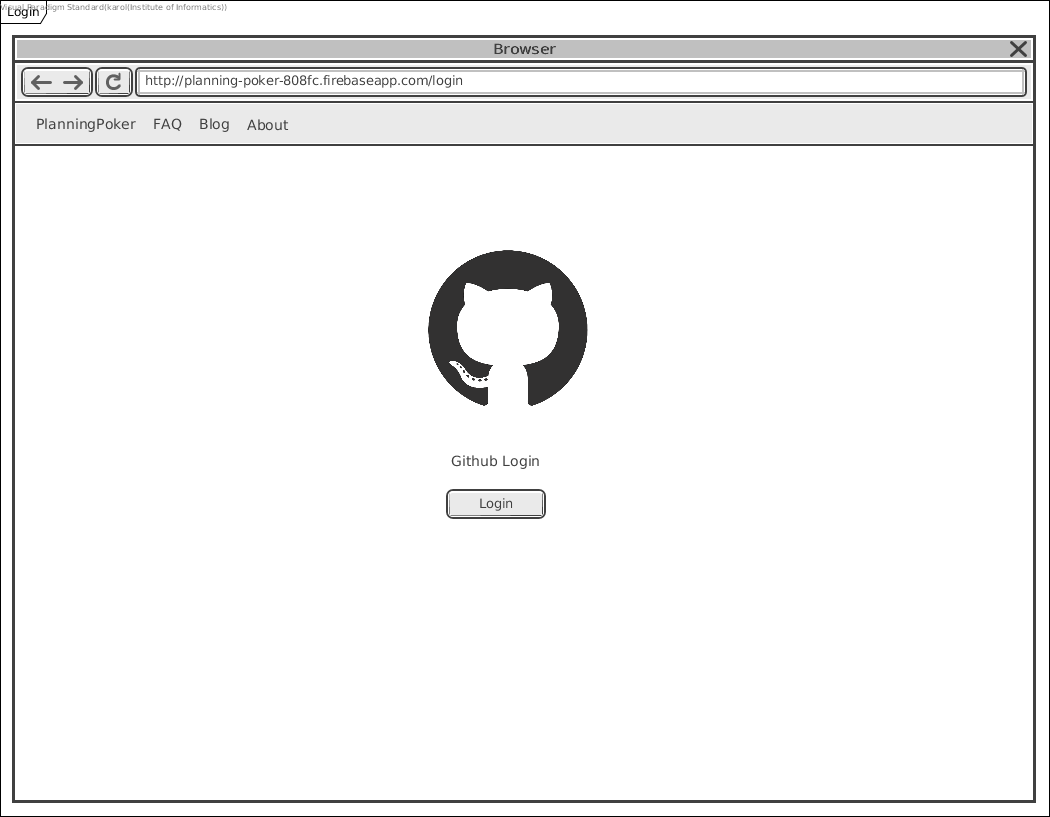
\includegraphics[width=.5\textwidth]{img/LoginScreen}
	\caption{Ekran Logowania}.
	\label{rys:loginScreen}
\end{figure}

\begin{figure}[h]
	\centering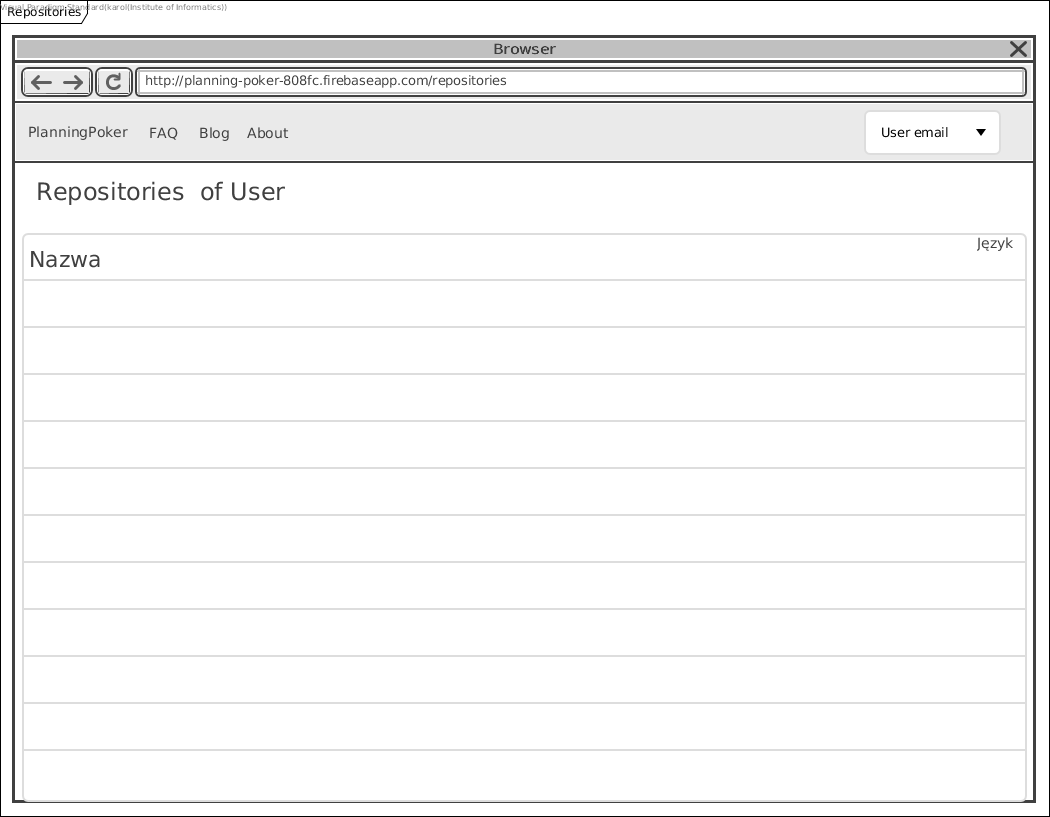
\includegraphics[width=.7\textwidth]{img/RepositoriesScreen}
	\caption{Ekran główny aplikacji z repozytoriami}.
	\label{rys:RepositoriesScreen}
\end{figure}

\begin{figure}[h]
	\centering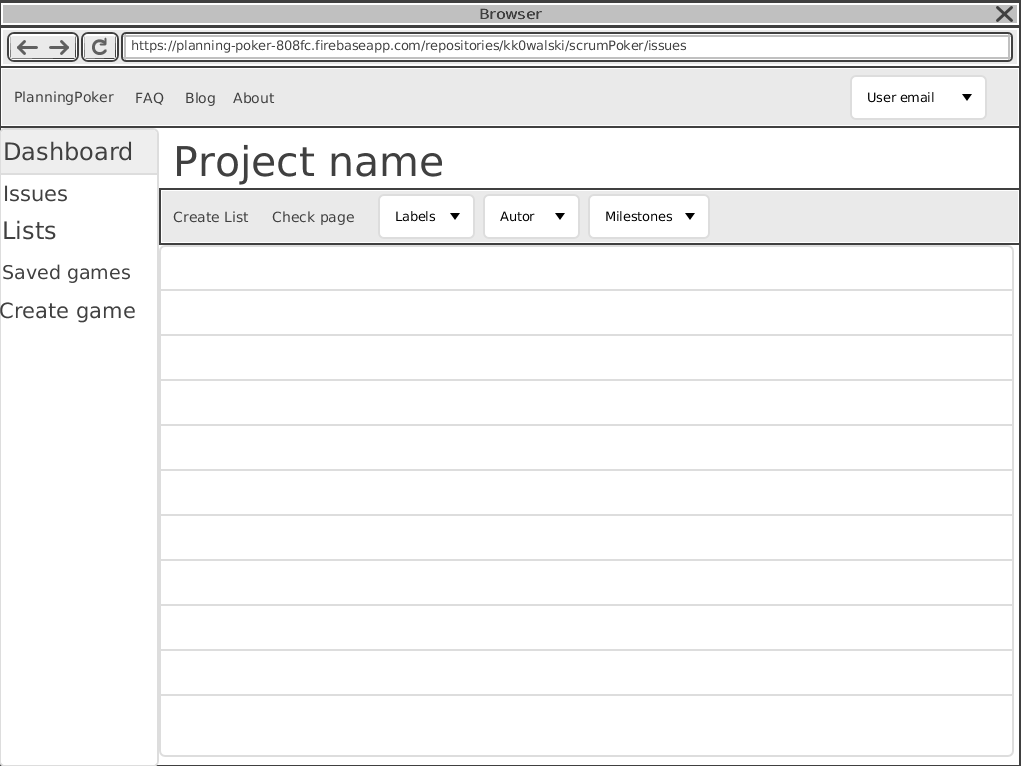
\includegraphics[width=.7\textwidth]{img/IssuesScreen}
	\caption{Główny ekran projektu}.
	\label{rys:IssuesScreen}
\end{figure}

\begin{figure}[h]
	\centering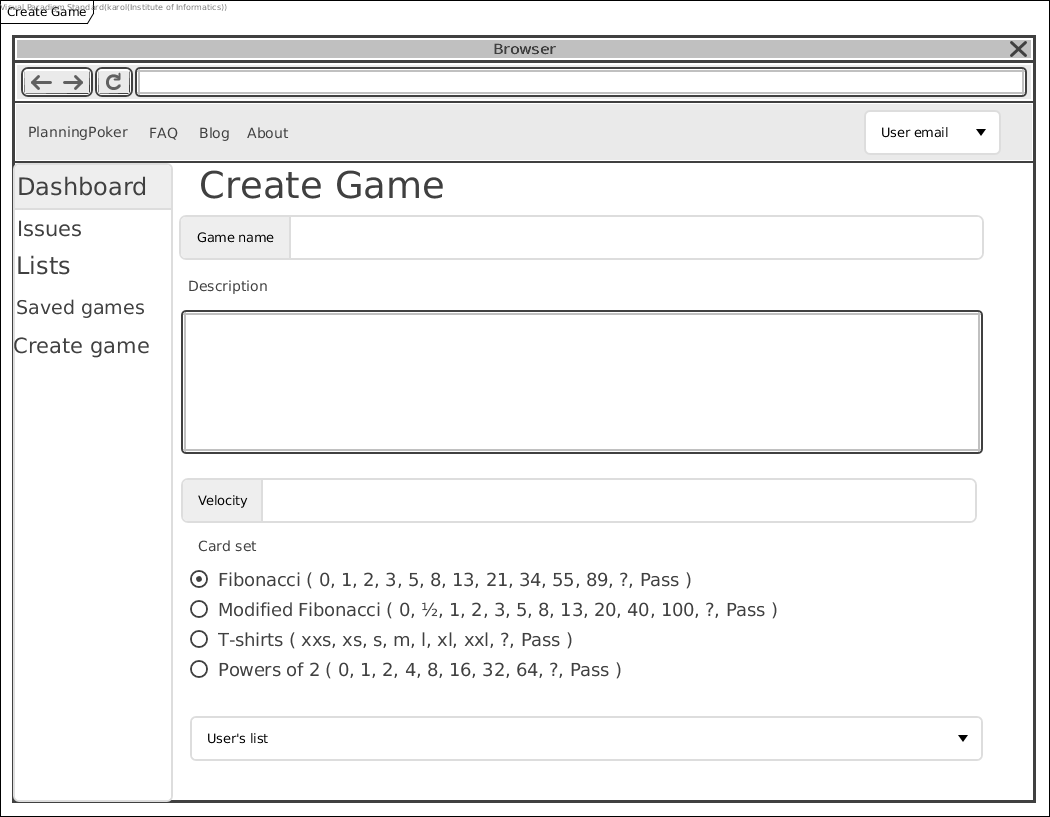
\includegraphics[width=.7\textwidth]{img/gameCreate}
	\caption{Formularz tworzenia gry}.
	\label{rys:gameCreate}
\end{figure}

\begin{figure}[h]
	\centering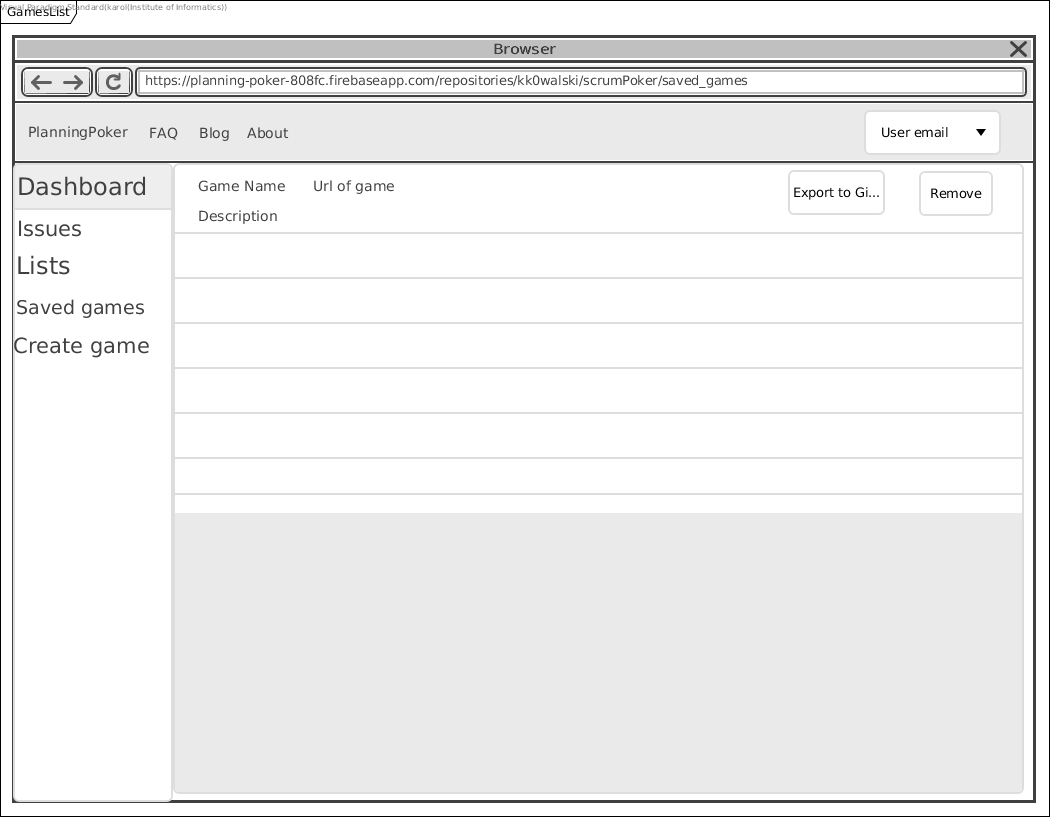
\includegraphics[width=.7\textwidth]{img/GamesList}
	\caption{Ekran gier}.
	\label{rys:GamesList}
\end{figure}

\begin{figure}[h]
	\centering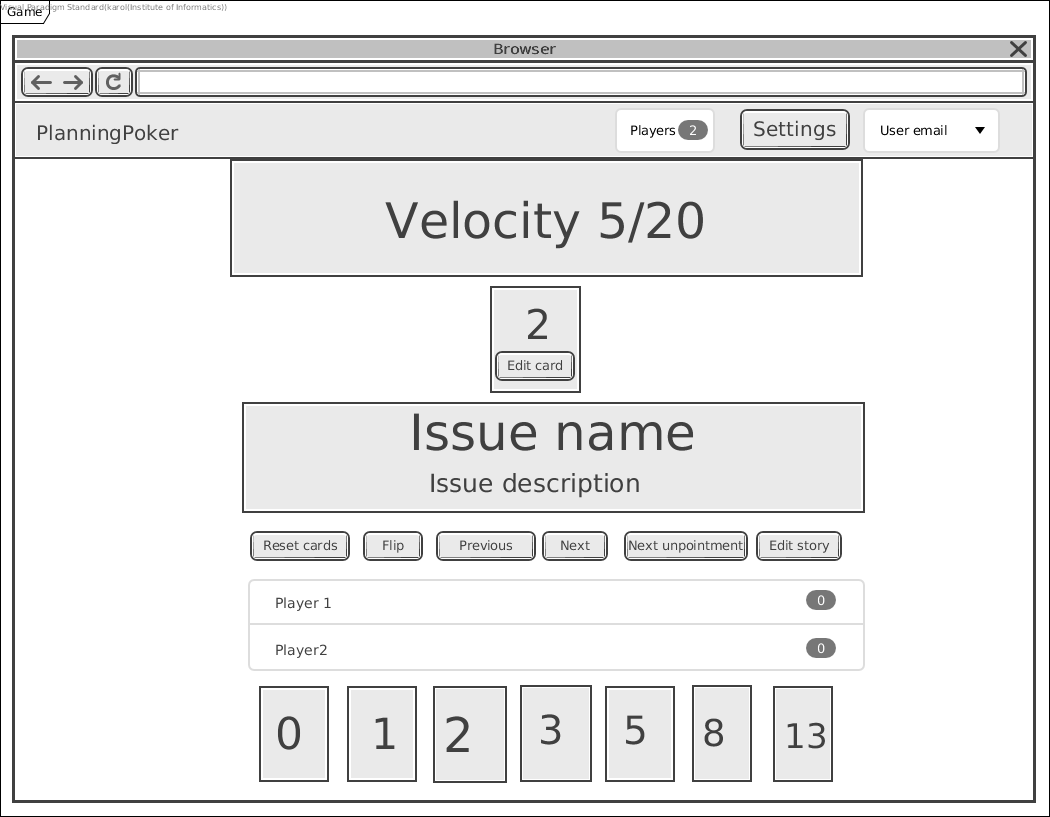
\includegraphics[width=.7\textwidth]{img/GameScreen}
	\caption{Panel gry}.
	\label{rys:GameScreen}
\end{figure}

\begin{figure}[h]
	\centering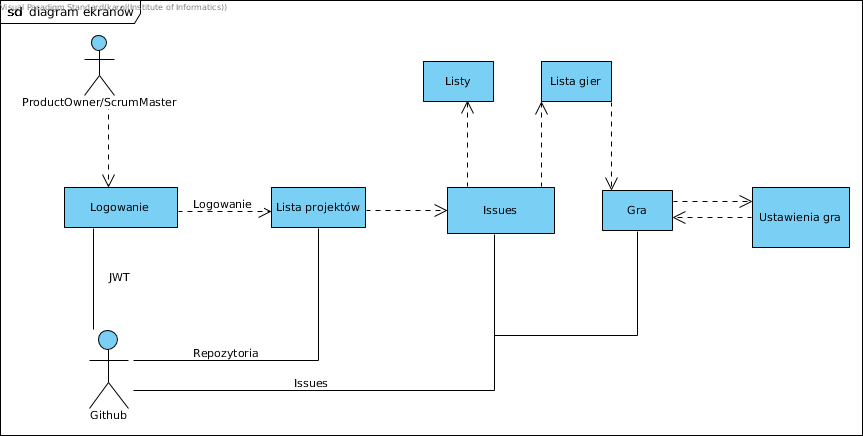
\includegraphics[width=.7\textwidth]{img/ScreensDiagram}
	\caption{Diagram przepływu między ekranami aplikacji}.
	\label{rys:ScreensDiagram}
\end{figure}

\section{Baza danych}

